\documentclass{beamer}

\usepackage{graphicx}
\usepackage{booktabs}
\usepackage[T1]{fontenc}
\usepackage{algorithm2e}
\usepackage{multimedia}
\usepackage{array}

\mode<presentation> {
	% \usetheme{default}
	% \usetheme{AnnArbor}
	% \usetheme{Antibes}
	% \usetheme{Bergen}
	% \usetheme{Berkeley}
	% \usetheme{Berlin}
	% \usetheme{Boadilla}
	% \usetheme{CambridgeUS}
	% \usetheme{Copenhagen}
	% \usetheme{Darmstadt}
	% \usetheme{Dresden}
	% \usetheme{Frankfurt}
	% \usetheme{Goettingen}
	% \usetheme{Hannover}
	% \usetheme{Ilmenau}
	% \usetheme{JuanLesPins}
	% \usetheme{Luebeck}
	\usetheme{Madrid}
	% \usetheme{Malmoe}
	% \usetheme{Marburg}
	% \usetheme{Montpellier}
	% \usetheme{PaloAlto}
	% \usetheme{Pittsburgh}
	% \usetheme{Rochester}
	% \usetheme{Singapore}
	% \usetheme{Szeged}
	% \usetheme{Warsaw}

	% \usecolortheme{albatross}
	% \usecolortheme{beaver}
	% \usecolortheme{beetle}
	% \usecolortheme{crane}
	% \usecolortheme{dolphin}
	% \usecolortheme{dove}
	% \usecolortheme{fly}
	% \usecolortheme{lily}
	% \usecolortheme{orchid}
	% \usecolortheme{rose}
	% \usecolortheme{seagull}
	\usecolortheme{seahorse}
	% \usecolortheme{whale}
	% \usecolortheme{wolverine}

	% \setbeamertemplate{footline} % To remove the footer line in all slides uncomment this line
	% \setbeamertemplate{footline}[page number] % To replace the footer line in all slides with a simple slide count uncomment this line
	% \setbeamertemplate{navigation symbols}{} % To remove the navigation symbols from the bottom of all slides uncomment this line
}

\AtBeginSection[]{
  \begin{frame}
    \frametitle{Contents}
    \tableofcontents[currentsection]
  \end{frame}
}
\AtBeginSubsection[]{
  \begin{frame}
    \frametitle{Contents}
    \tableofcontents[currentsubsection]
  \end{frame}
}
\AtBeginSubsubsection[]{
  \begin{frame}
	\frametitle{Contents}
	\tableofcontents[currentsubsection]
  \end{frame}
}

\title[Projet de Fin d'Étude]{Projet de Fin d'Étude}
\author{Brandon Alves}
\institute[INSA Lyon]{
	\huge{Réunion de mi-parcours}
}

\date{\today}

\begin{document}
	\begin{frame}
		\titlepage
	\end{frame}
	\begin{frame}
		\frametitle{Contents}
		\tableofcontents
	\end{frame}
	\section{Contexte}
		\begin{frame}
			\frametitle{Contexte}
			\begin{itemize}
				\item Projet européen BugWright2
				\item Inspection de structures métalliques
				\item Tomographie de la zone à inspecter
				\item Localiser des points de corrosion
			\end{itemize}
		\end{frame}
		\begin{frame}
			\frametitle{Contexte}
			\begin{figure}
				\centering
				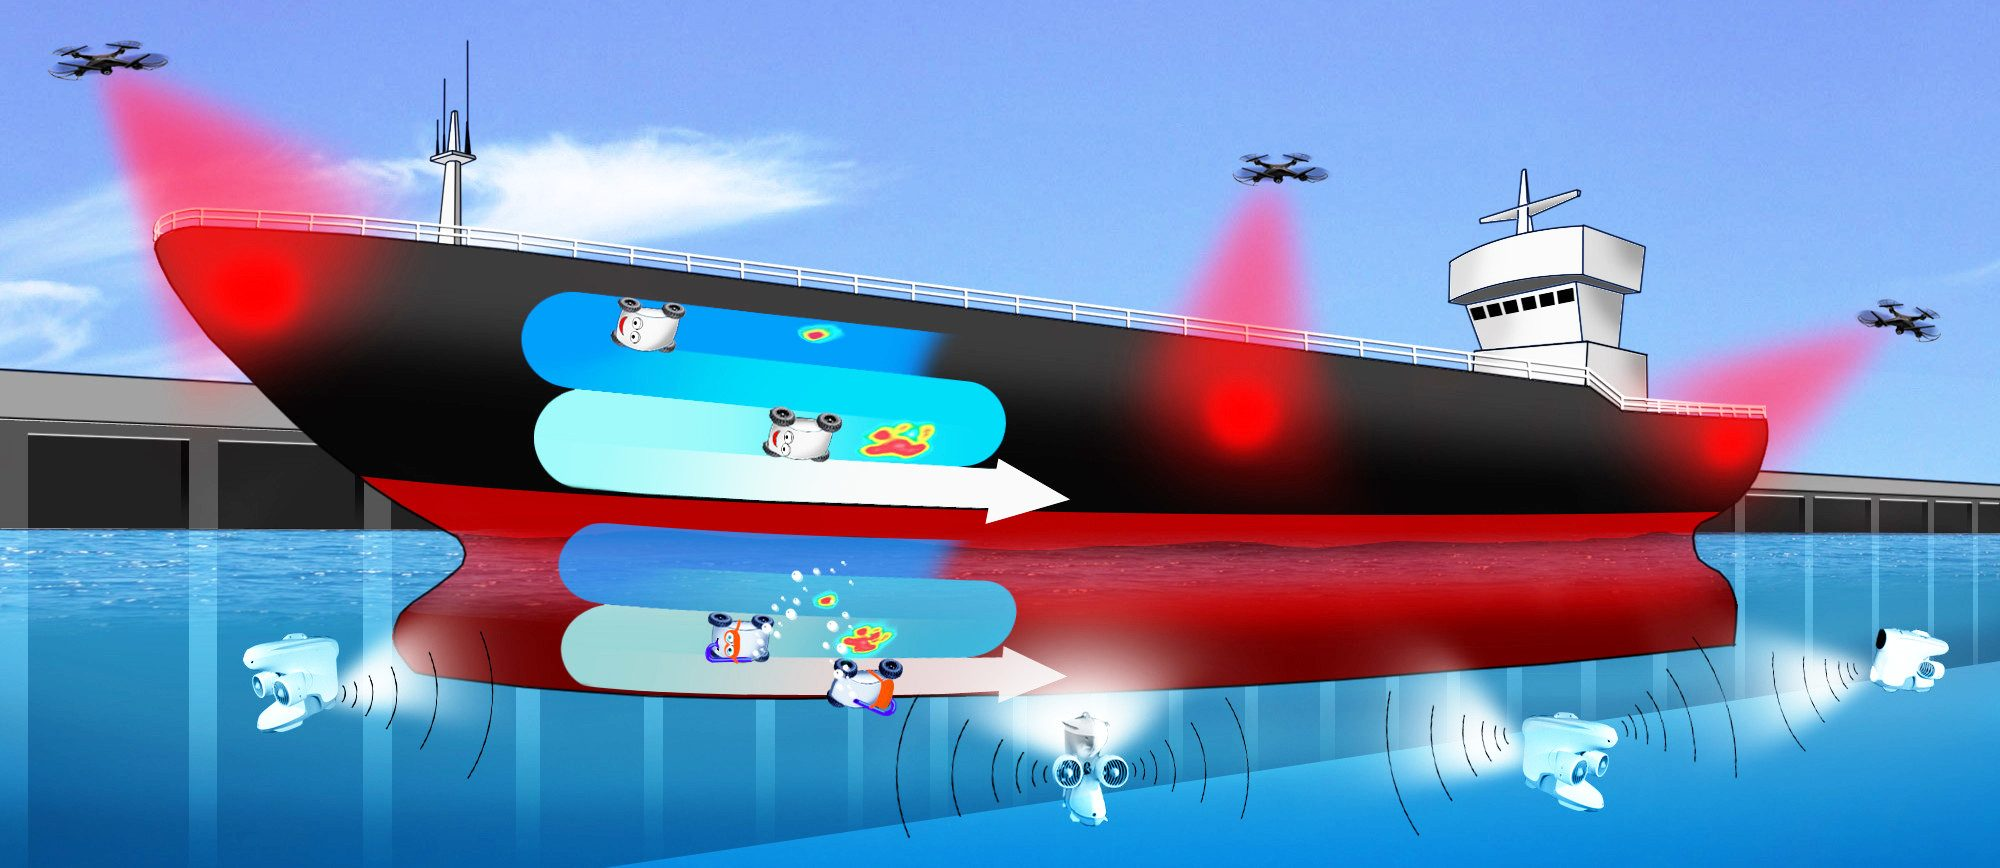
\includegraphics[width=0.8\textwidth]{graphics/Concept-Cartoon-NJ3-e1582812224528.jpg}
				\caption{Projet BugWright2 (https://www.bugwright2.eu/project/)}
			\end{figure}
		\end{frame}
	\section{Problème \& hypothèses}
		\begin{frame}
			\frametitle{Problème \& hypothèses}
			\begin{block}{Problème}
				Définir des stratégies de navigation multi-robot pour optimiser l'acquisition de données permettant de réaliser la tomographie des structures métalliques.
			\end{block}
		\end{frame}
		\begin{frame}
			\frametitle{Problème \& hypothèses}
			\begin{block}{Hypothèses}
				\begin{itemize}
					\item Environnement :
					\begin{itemize}
						\item espace 2D, borné et de taille connue,
						\item obstacles localisés,
						\item zones de corrosion non localisées.
					\end{itemize}
					\item Robots :
					\begin{itemize}
						\item robots à 2 roues,
						\item pose $(x, y, \theta)$ connue,
						\item coût de rotation $cr$ et coût de translation $ct$ connus.
						\item Nombre de robots $\ge$ 2.
					\end{itemize}
					\item Perception :
					\begin{itemize}
						\item Robot est émetteur ou récepteur,
						\item Émission et réception omnidirectionnelle d'ondes ultrasoniques (\textit{UGW}),
						\item Si puissance de signal altérée, alors détection,
						\item Détection parfaite et en temps réel,
						\item Distance maximale d'émission et de réception $d_{max}$.
					\end{itemize}
				\end{itemize}
			\end{block}
		\end{frame}
		\begin{frame}
			\frametitle{Problème \& hypothèses}
			\begin{block}{Structures de données}
				\begin{itemize}
					\item Grille d'occupation :
					\begin{itemize}
						\item inconnu,
						\item vide,
						\item occupé.
					\end{itemize}
				\end{itemize}
			\end{block}
		\end{frame}
	\section{Stratégies de navigation}
		\subsection{Stratégies}
			\begin{frame}
				\frametitle{Stratégies}
				\begin{block}{Strétégies de navigation}
					\begin{itemize}
						\item Stratégies de navigation grossières,
						\item Investigation polygonale.
					\end{itemize}
				\end{block}
				\begin{block}{Hypothèse}
					\begin{itemize}
						\item Formes convexes.
					\end{itemize}
				\end{block}
			\end{frame}
		\subsection{Stratégies de navigation grossières}
			\subsubsection{Peinture au rouleau}
				\begin{frame}
					\frametitle{Stratégies de navigation grossières}
					\framesubtitle{Peinture au rouleau}
					\begin{block}{Description}
						\begin{itemize}
							\item Nombre de robots $\ge$ 2,
							\item Chaque robot se déplace en ligne droite,
							\item Les robots se déplacent en parallèle,
							\item Les robots se synchronisent régulièrment.
						\end{itemize}
					\end{block}
				\end{frame}
				\begin{frame}
					\frametitle{Stratégies de navigation grossières}
					\framesubtitle{Peinture au rouleau}
					\begin{figure}
						\centering
						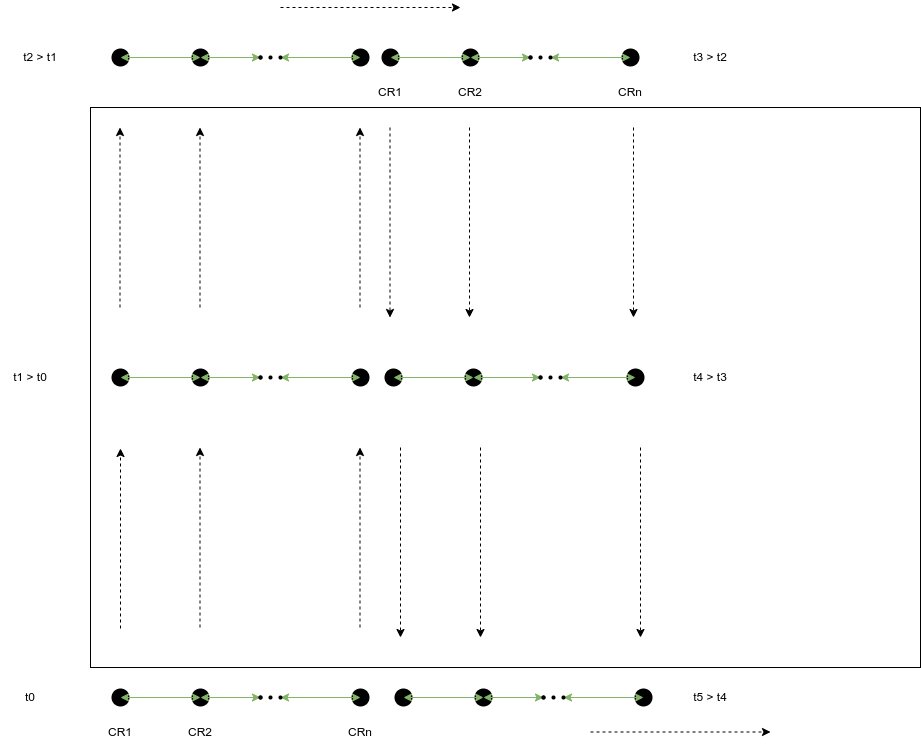
\includegraphics[width=0.6\textwidth]{graphics/peinture_au_rouleau1.png}
						\caption{Peinture au rouleau - passe verticale}
					\end{figure}
				\end{frame}
				\begin{frame}
					\frametitle{Stratégies de navigation grossières}
					\framesubtitle{Peinture au rouleau}
					\begin{figure}
						\centering
						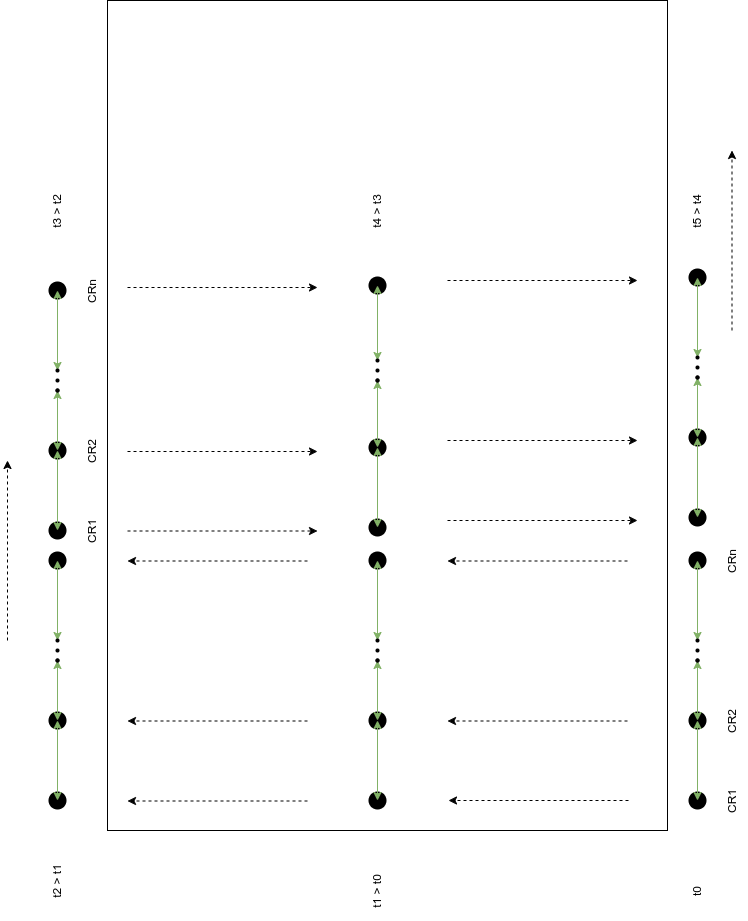
\includegraphics[width=0.4\textwidth]{graphics/peinture_au_rouleau2.png}
						\caption{Peinture au rouleau - passe horizontale}
					\end{figure}
				\end{frame}
				\begin{frame}
					\frametitle{Stratégies de navigation grossières}
					\framesubtitle{Peinture au rouleau}
					\begin{figure}[H]
						\centering
						\movie[label=show1, poster, showcontrols]{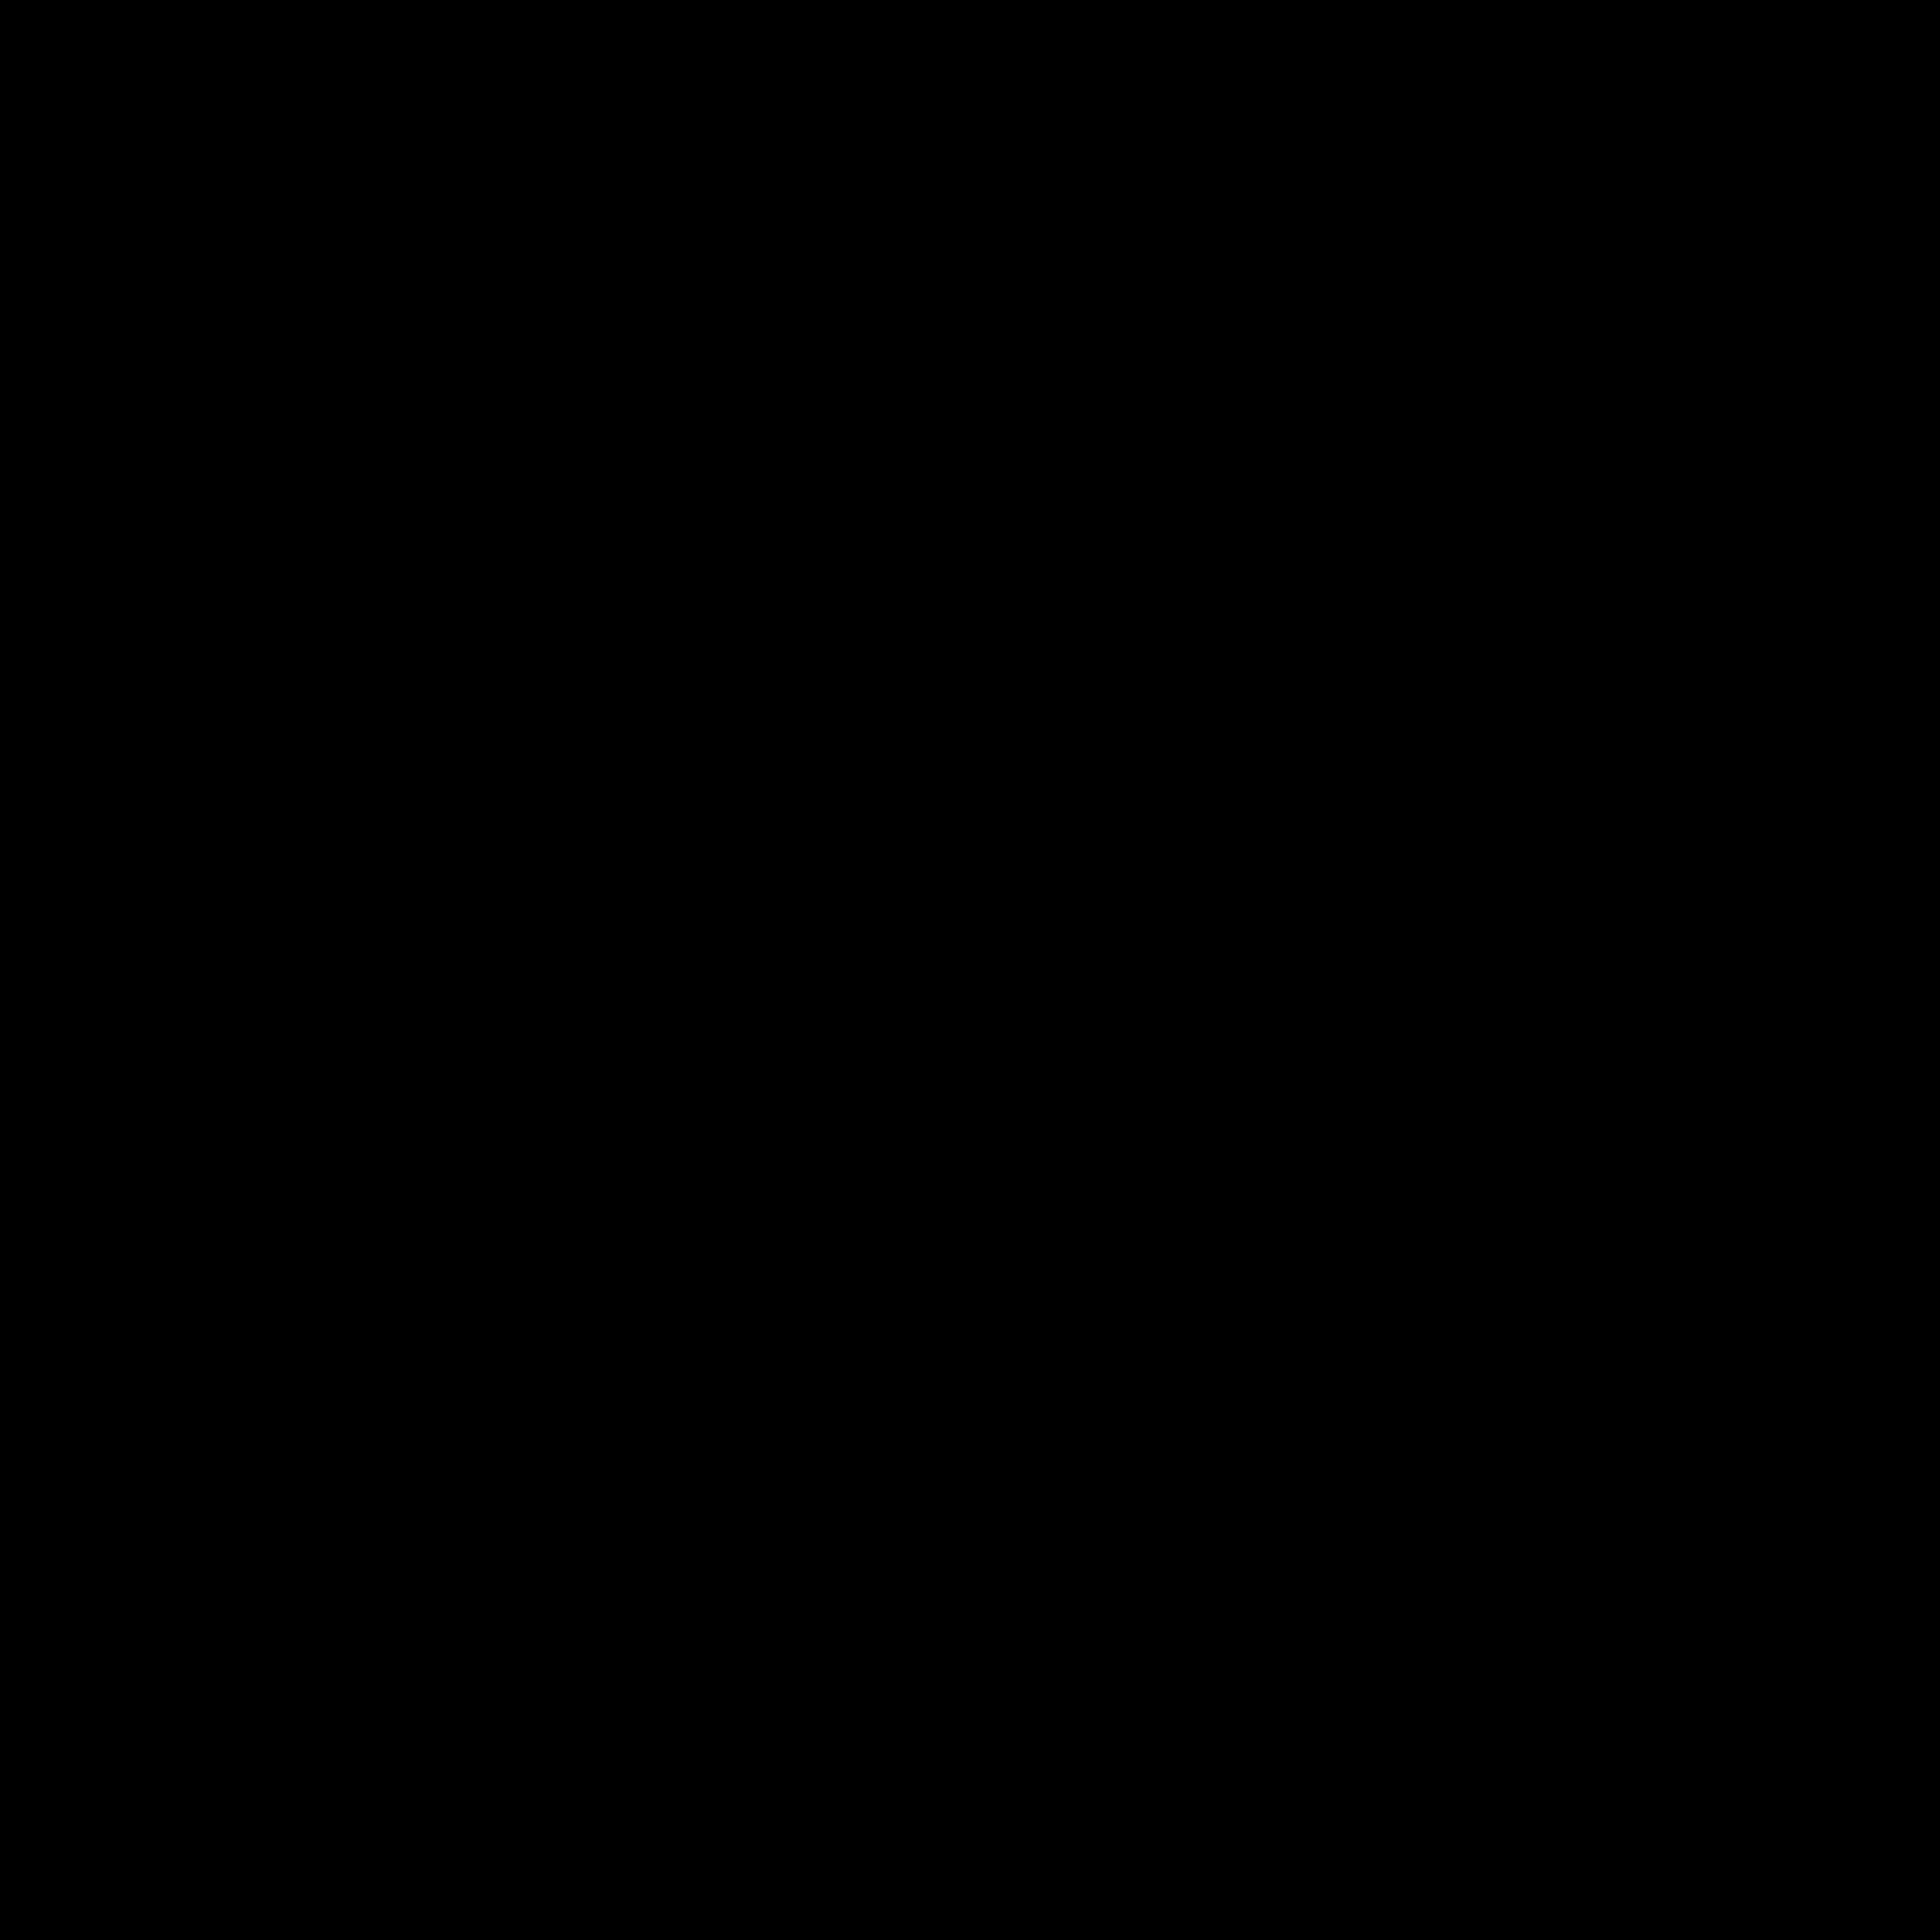
\includegraphics[scale=0.08]{graphics/black.png}}{graphics/d=2.0_o=0.1_v=0.2.mp4}
						\caption{Peinture au rouleau, d=4.0, o=0.1, v=0.3}
					\end{figure}
				\end{frame}
				\begin{frame}
					\frametitle{Stratégies de navigation grossières}
					\framesubtitle{Peinture au rouleau}
					\begin{exampleblock}{Avantages}
						\begin{itemize}
							\item Simple à mettre en oeuvre,
							\item Peut être utilisé pour des zones de tailles importantes,
							\item Rapide.
						\end{itemize}
					\end{exampleblock}
					\begin{alertblock}{Inconvénients}
						\begin{itemize}
							\item Enveloppe rectangulaire,
							\item Peu précis,
							\item Zones fantômes.
						\end{itemize}
					\end{alertblock}
				\end{frame}
			\subsubsection{Ski nordique}
				\begin{frame}
					\frametitle{Stratégies de navigation grossières}
					\framesubtitle{Ski nordique}
					\begin{block}{Description}
						\begin{itemize}
							\item Nombre de robots $\ge$ 2,
							\item Chaque robot se déplace en ligne droite,
							\item La trajectoire des robots est parallèle,
							\item Les robots se déplacent de manière asynchrone.
						\end{itemize}
					\end{block}
				\end{frame}
				\begin{frame}
					\frametitle{Stratégies de navigation grossières}
					\framesubtitle{Ski nordique}
					\begin{figure}
						\centering
						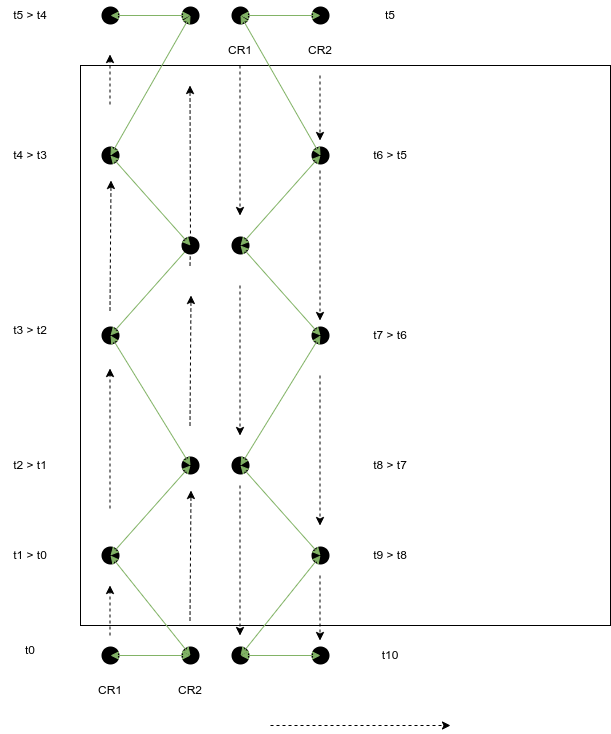
\includegraphics[width=0.4\textwidth]{graphics/ski_nordique1.png}
						\caption{Ski nordique - passe verticale}
					\end{figure}
				\end{frame}
				\begin{frame}
					\frametitle{Stratégies de navigation grossières}
					\framesubtitle{Ski nordique}
					\begin{figure}
						\centering
						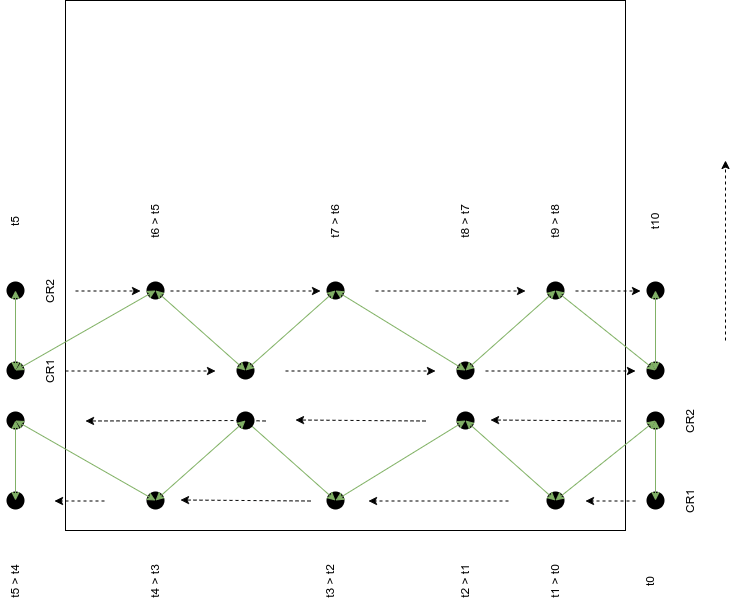
\includegraphics[width=0.6\textwidth]{graphics/ski_nordique2.png}
						\caption{Ski Nordique - passe horizontale}
					\end{figure}
				\end{frame}
				\begin{frame}<0>
					\frametitle{Stratégies de navigation grossières}
					\framesubtitle{Peinture au rouleau}
					\begin{figure}[H]
						\centering
						\movie[label=show1, poster, showcontrols]{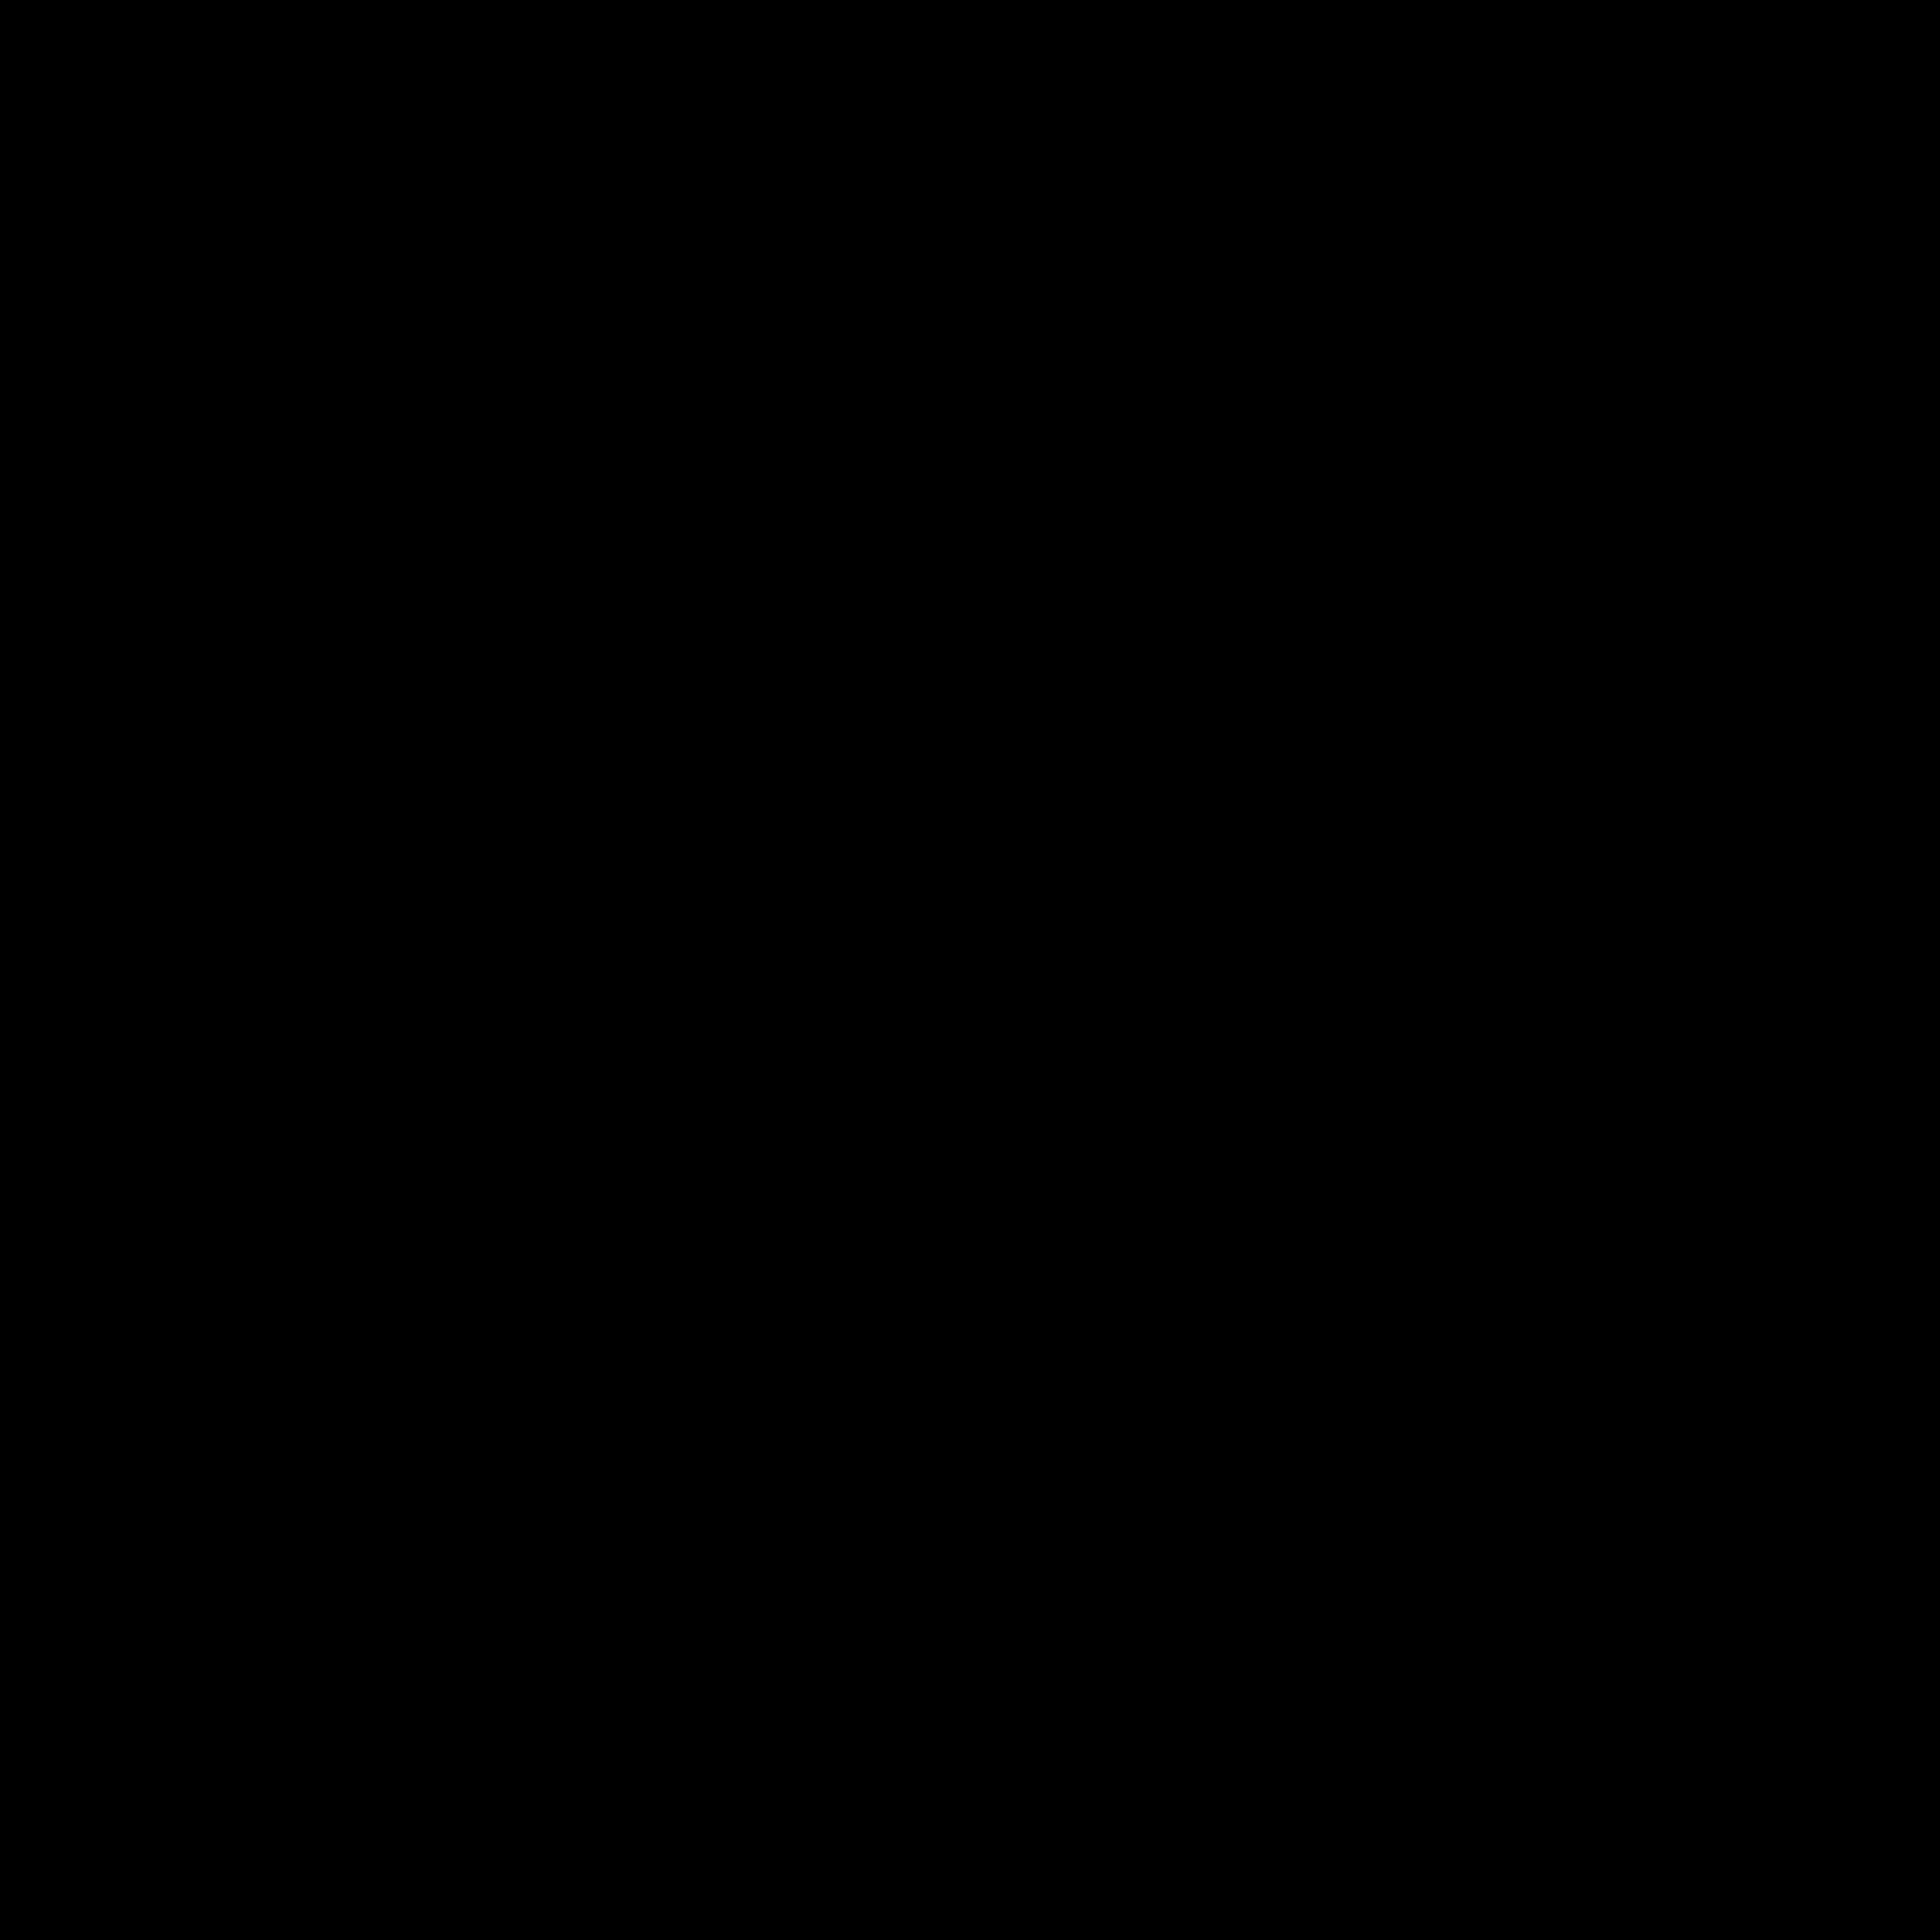
\includegraphics[scale=0.08]{graphics/black.png}}{graphics/ski_nordique.mp4}
						\caption{Peinture au rouleau, d=4.0, o=0.1, v=0.3}
					\end{figure}
				\end{frame}
				\begin{frame}
					\frametitle{Stratégies de navigation grossières}
					\framesubtitle{Ski nordique}
					\begin{exampleblock}{Avantages comparé à peinture au rouleau}
						\begin{itemize}
							\item Enveloppe d'un polygone convexe à $4$ côtés,
							\item Peut être utilisé pour des zones de tailles importantes,
							\item Plus précis que la peinture au rouleau.
						\end{itemize}
					\end{exampleblock}
					\begin{alertblock}{Inconvénients comparé à peinture au rouleau}
						\begin{itemize}
							\item Moins simple à mettre en oeuvre,
							\item Plus lent que la peinture au rouleau,
							\item Zones fantômes.
						\end{itemize}
					\end{alertblock}
				\end{frame}
		\subsection{Investigation polygonale}
			\begin{frame}
				\frametitle{Investigation polygonale}
				\begin{block}{Description}
					\begin{itemize}
						\item $k \ge 1$ équipes de $n \ge 2$ robots,
						\item Les robots d'une même équipe se placent sur des sommets consécutifs d'un polygone convexe,
						\item Les robots se déplacent l'un après l'autre.
					\end{itemize}
				\end{block}
			\end{frame}
			\begin{frame}
				\frametitle{Investigation polygonale}
				\begin{figure}
					\centering
					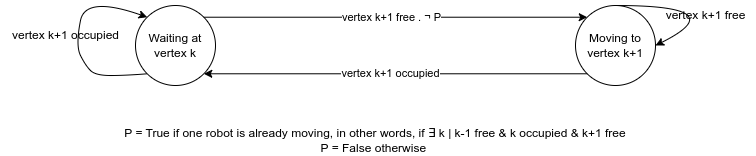
\includegraphics[width=1.0\textwidth]{graphics/automat_poly.png}
					\caption{Automate à états finis pour un robot lors d'une investigation polygonale}
				\end{figure}
			\end{frame}
			\begin{frame}
				\frametitle{Investigation polygonale}
				\begin{figure}[H]
					\centering
					\movie[label=show1, poster, showcontrols]{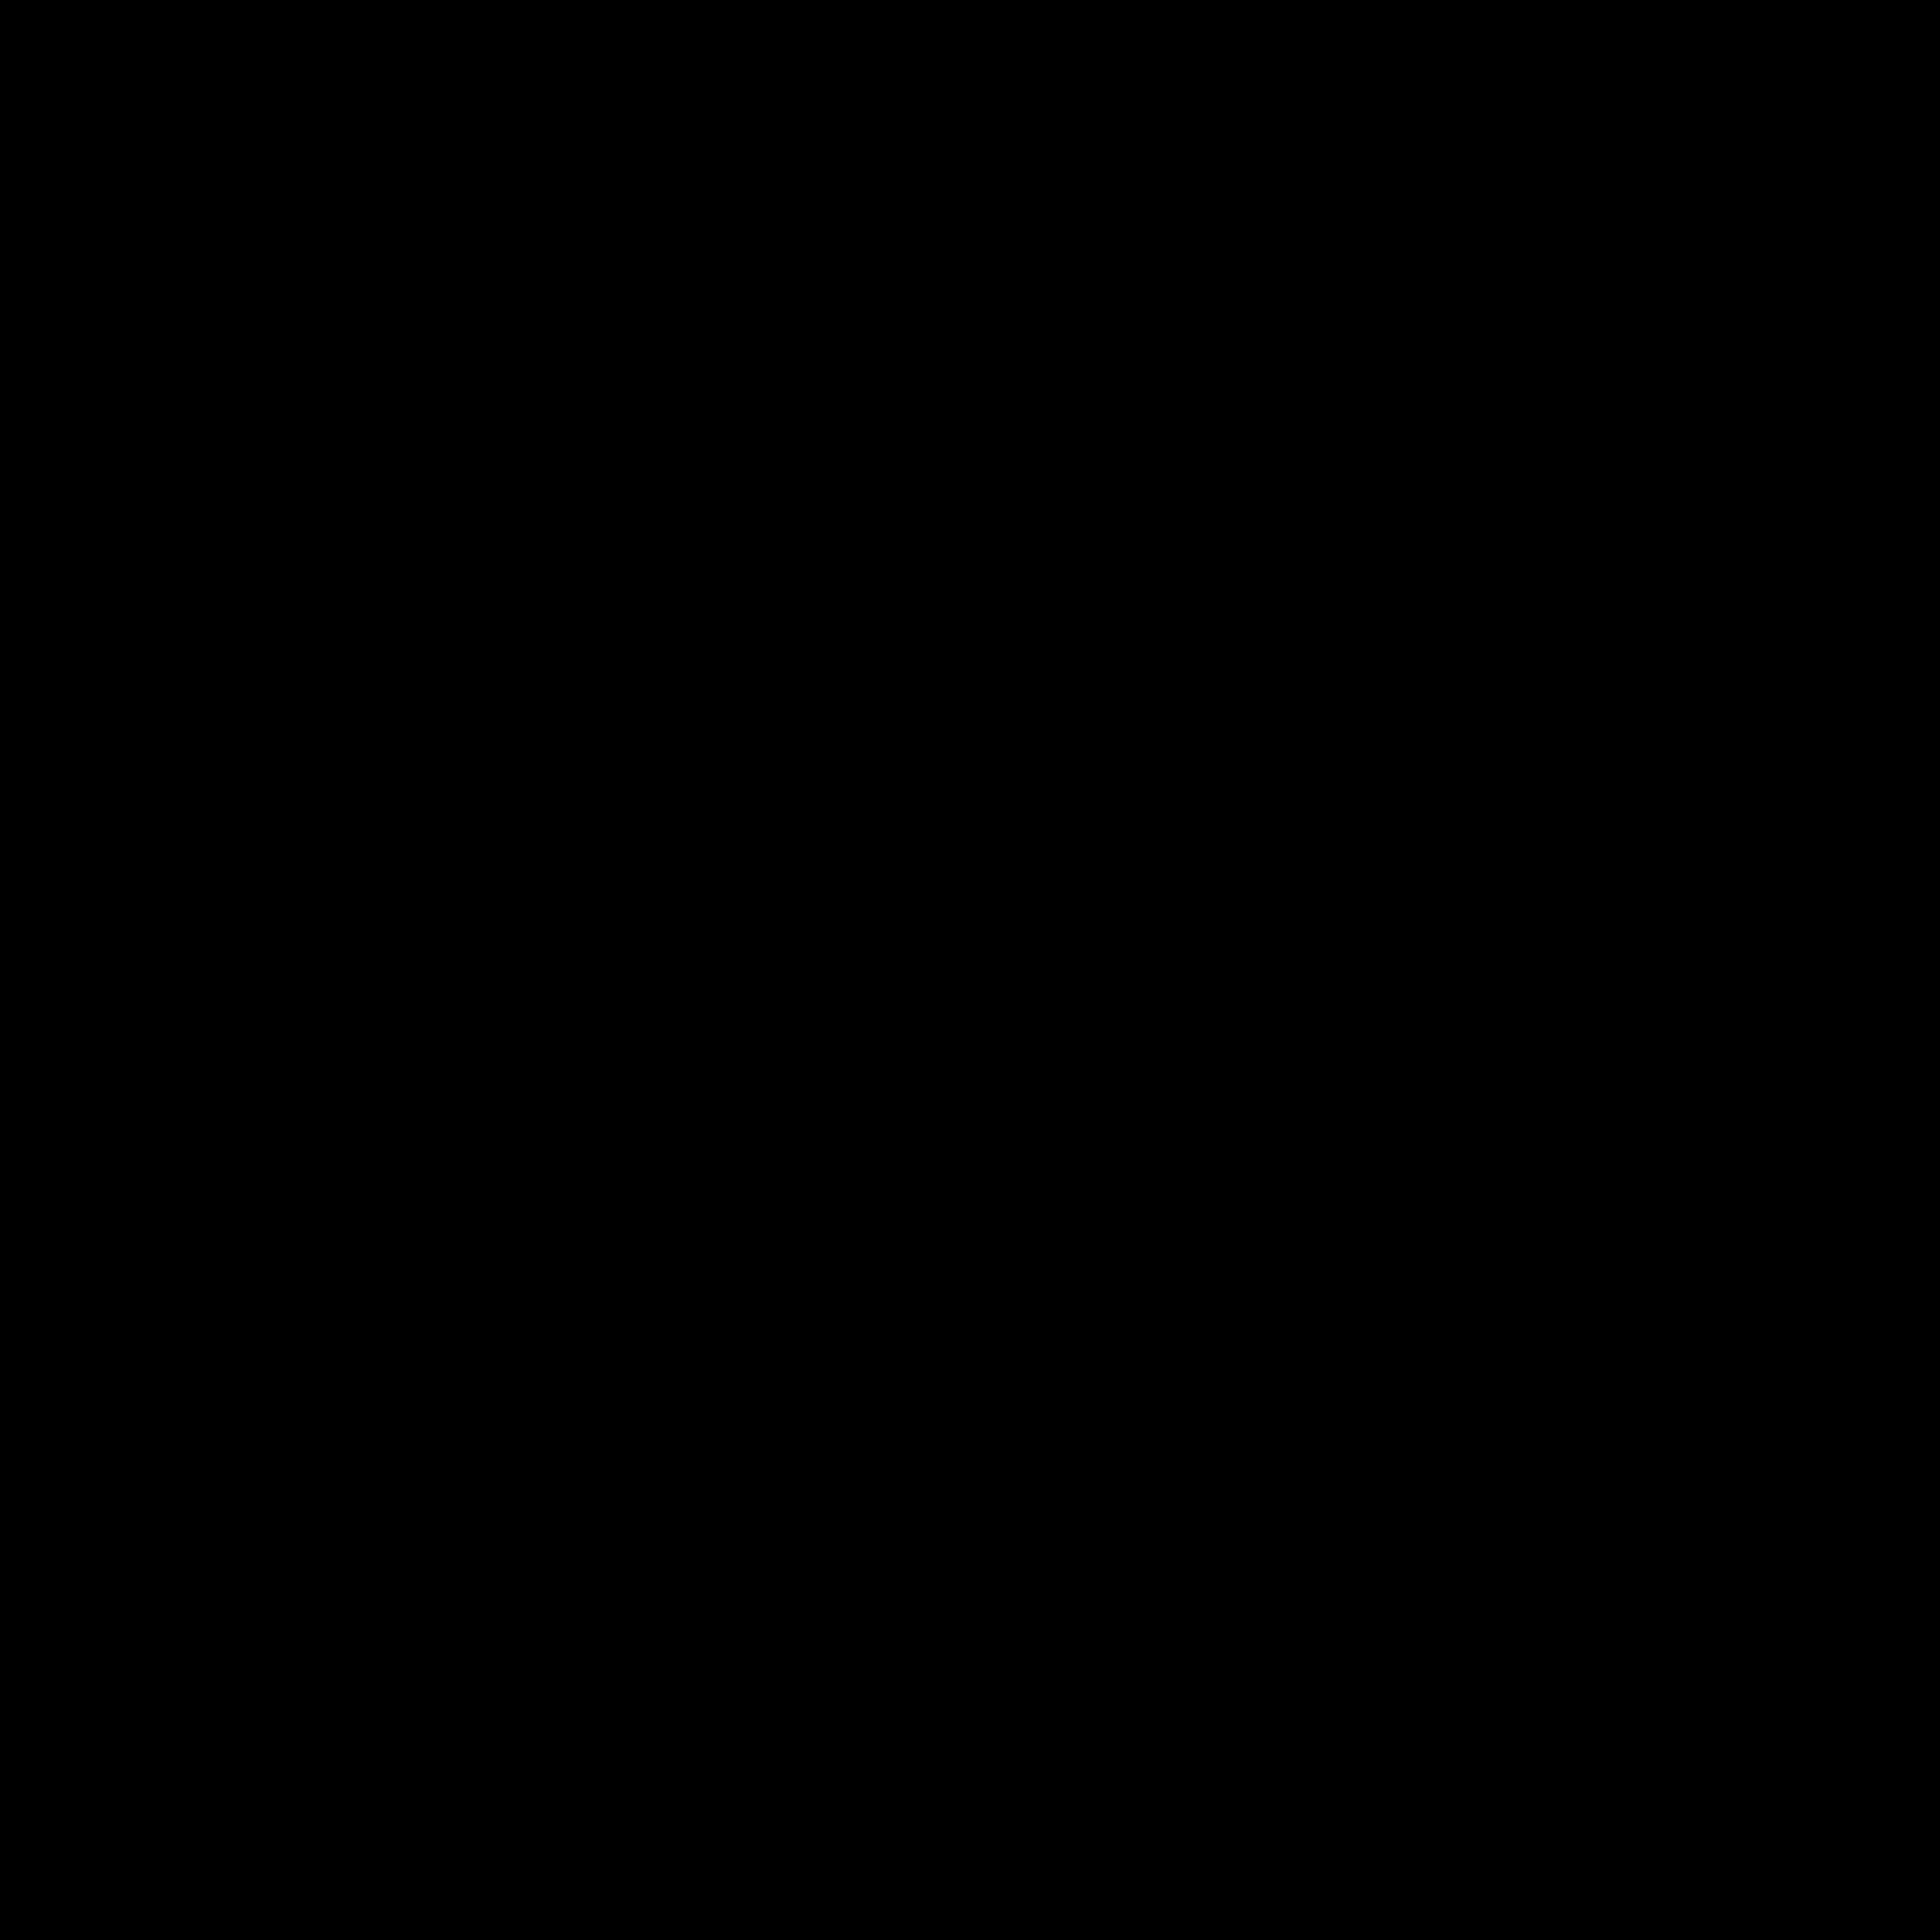
\includegraphics[scale=0.08]{graphics/black.png}}{graphics/invest.mp4}
					\caption{Peinture au rouleau, d=4.0, o=0.1, v=0.3}
				\end{figure}
			\end{frame}
			\begin{frame}
				\frametitle{Investigation polygonale}
				\begin{exampleblock}{Avantages}
					\begin{itemize}
						\item Niveau de précision variable de l'enveloppe convexe de la zone de corrosion (proportionnellement au nombre de sommet du polygone)
						\item Efficace pour des zones de petites tailles,
						\item Permet de rapidement éliminer les zones fantômes.
					\end{itemize}
				\end{exampleblock}
				\begin{alertblock}{Inconvénients}
					\begin{itemize}
						\item Lent (proportionnellement au nombre de sommet du polygone, inversement proportionnel au nombre de robots),
					\end{itemize}
				\end{alertblock}
			\end{frame}
		\subsection{Scénario}
			\begin{frame}
				\frametitle{Scénario}
				\begin{enumerate}
					\item Peinture au rouleau
					\item Extraction des zones de corrosion
					\item Calcul des centroides et des polygones
					\item Resolution du mTSP connectant les centroides
					\item Investigation polygonale
				\end{enumerate}
			\end{frame}
	\section{Évaluation}
		\begin{frame}
			\frametitle{Métrique de performance}
			Kappa de Cohen:
			\begin{equation*}
				\kappa = \frac{p_o - p_e}{1 - p_e}
			\end{equation*}
			avec :
			\begin{itemize}
				\item $p_o$ : précision observée,
				\item $p_e$ : précision aléatoire,
				\item $\kappa$ : mesure une classification binaire, en la comparant à une classification aléatoire.
			\end{itemize}
			\begin{table}
				\centering
				\begin{tabular}{|c|c|}
					\hline
					$\kappa$ & Interprétation \\
					\hline
					$< 0$ & Désaccord \\
					\hline
					$0.00 - 0.20$ & Accord très faible \\
					\hline
					$0.21 - 0.40$ & Accord faible \\
					\hline
					$0.41 - 0.60$ & Accord modéré \\
					\hline
					$0.61 - 0.80$ & Accord fort \\
					\hline
					$0.81 - 1.00$ & Accord presque parfait \\
					\hline
				\end{tabular}
				\caption{Interprétation du $\kappa$ de Cohen selon Landis et Koch}
			\end{table}
		\end{frame}
		\begin{frame}
			\frametitle{Résultats}
			\framesubtitle{Peinture au rouleau}
			\begin{figure}
				\centering
				
\includegraphics[scale=1.0]{graphics/d=2.0_o=0.1_v=0.2.png}
				\caption{Peinture au rouleau, d = 2.0m, o = 0.1m, v = 0.2m/s}
			\end{figure}
			Score : $\kappa = 0.63$, Temps : $t = 9 \text{min} 4 \text{sec}$
		\end{frame}
		\begin{frame}
			\frametitle{Résultats}
			\framesubtitle{Peinture au rouleau}
			\begin{figure}
				\centering
				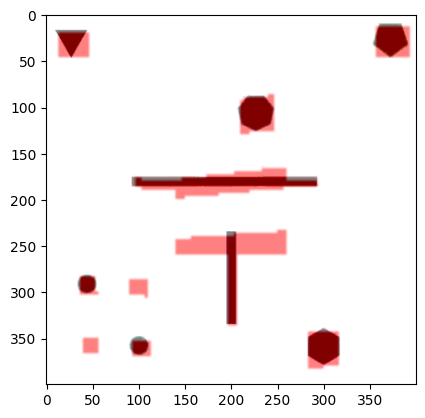
\includegraphics[scale=0.5]{graphics/result.png}
				\caption{Résultat peinture au rouleau, d = 2.0m, o = 0.1m, v = 0.2m/s}
			\end{figure}
			Score : $\kappa = 0.63$, Temps : $t = 9 \text{min} 4 \text{sec}$
		\end{frame}
		\begin{frame}
			\frametitle{Résultats}
			\framesubtitle{Investigation polygonale}
			\begin{figure}
				\centering
				
\includegraphics[scale=1.0]{graphics/occupancy_grid.png}
				\caption{Investigation polygonale, p = 4, n = 2}
			\end{figure}
			Score : $\kappa = 0.66$
		\end{frame}
		\begin{frame}
			\frametitle{Résultats}
			\framesubtitle{Peinture au rouleau}
			\begin{figure}
				\centering
				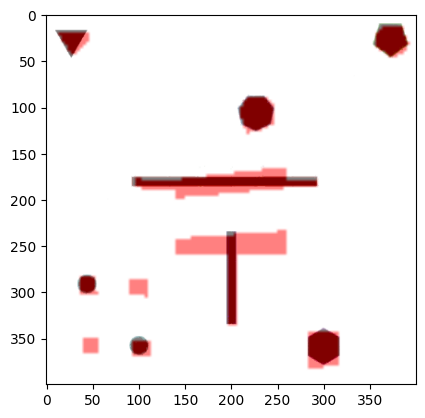
\includegraphics[scale=0.5]{graphics/output.png}
				\caption{Résultat peinture au rouleau, d = 2.0m, o = 0.1m, v = 0.2m/s}
			\end{figure}
			Score : $\kappa = 0.63$
		\end{frame}
	\section{Conclusion}
		\begin{frame}
			\frametitle{Conclusion}
			% Choses qu'il reste à faire
		\end{frame}
\end{document}
